\section{ SR0015US22 }


\subsection{Meta}

    \textbf{Title:}
    Stochastic optimization approaches for elective surgery scheduling with downstream capacity constraints: Models, challenges, and opportunities

    \begin{table}[H]
        \centering
        \begin{tabular}{|c|c|c|c|c|c|c|c|c|}
            \hline
                \textbf{Rank} & \textbf{Grasp} & \textbf{Grade} & \textbf{Type} & \textbf{Outcome} & \textbf{Domain} & \textbf{COV19} & \textbf{CoI} & \textbf{DB} \\
            \hline
                5 & 84\% & A+ & A & P & B & Yes & ?? & Yes \\
            \hline
        \end{tabular}
        \caption{Reference's metadata}
        \label{tab:SR02CN23}
    \end{table}

\subsection{Summary}
    Karmel S. Shehadeh and Rema Padma \cite{x335} propose a complex literature review on stochastic optimisation approaches for elective surgery scheduling with downstream capacities. The review focuses on three solution approaches from January 2010 to November 2020: Stochastic Optimisation (SO), Robust Optimisation (RO), and Distributionally Robust Optimisation. The importance of the research is stated, and the statements were supported with statistical data about the value of the operating theatres and the downstream capacities in hospitals. In the body of the paper, the authors describe individual parts of elective surgery scheduling, explain interconnections among constraints, and discuss the mathematical interpretations of the SO, RO, and DRO solutions. The examples of the solutions in other studies were demonstrated and discussed. The language in the research is addressed to advanced readers with sometimes excessive terminology. The paper proposed multiple suggestions on how it is possible to improve existing solutions and outlined further research areas. In conclusion, this literature review presents high-quality qualitative research with practical guidelines and in-depth knowledge of the researched field.   

\subsection{Notes}
    \begin{itemize}
        \item Starts with quotations;
        \item OR 40\%-70\% revenue (refs);
        \item OR 20\%-40\% operating costs (refs);
        \item SICU 15\%-40\% hospital costs (refs);
        \item Agency for Healthcare Research and Quality (AHRQ);
        \item 17.2 million hospital visits in 2014;
        \item Patients require surgery: 60\%-70\%;
        \item Specific way of useing "multi-modal";
        \item Healthcare in formation technologies (HIT);
        \item SO, RO, and DRO (Jan2010-Nov2020);
        \item Cost of cancelled case ~\$1700-\$2000, Argo et al.(2009);
        \item 15\% of cancellations ~lack of recovery beds;
        \item Survival rate SICU = noSICU x 6; 
        \item Data of the Erasmus University Medical Center;
        \item Real-time location system (RTLS);
        \item Advanced technical, specialised language;
        \item Goh, J., Sim, M., 2010. Distributionally robust optimization and its tractable approximations. Oper. Res. 58 (4-part-1), 902–917;
        \item Written with the reader in mind;
        \item Waht is Mig-M?
        \item Contains valuable references;
        \item E-HOSPITAL workbench;
    \end{itemize}


\subsection{Reading}
    \textbf{Abstract:}
    The flow of surgery operation with downstream capacity was explained. The authors conducted a review on existing solutions with focus on Stochastic Optimisation. The description of the processe of solving elective surgery scheduling was provided together with the suggestions for creating "tractable, implementable, and data-driven" solution methods.
    
    \textbf{Objectives:}
    Motivated by research collaboration with a large health system in Pennsylvania.
    
    \textbf{Page 1 (Quotations):}
    \textit{‘‘Each of the uncertainty veils carries a secret promise for creative mathematical art.’’} - Dr. Karmel S. Shehadeh (2021)
    
    \textit{‘‘Problems worthy of attack prove their worth by hitting back.’’} – Piet Hein, Grooks (1966)

    \textbf{Page 1 (Introduction):}
    The authors backed the value of operating rooms by showing the numbers of the revenue it produces of amoung all hospital sources, and costs it requires in porcentile to all hospital expances. The description of OR scehduling and introduction of the three decision stages are stated next.
    
    \textbf{Page 2 (Introduction):}
    Three levels: strategic, tactical, and operational. Operational splits further into advance and allocation scheduling. The stochastic nature of the surgery scheduling problem such as operation duration and lenght-of-stay (LOS) raise additional obsticle on the way of optimal operating room usega. The normal distribution do not fully reflect the real fluctuation of the surgery durations. Multi-modal = multi-modality = bimodal = bimodality = not unimodal = not fully known. Lack of information leads to inefficient OR utilisation. The OR scheduling with downstream capacity is a special case of "stichastic hybrid flow shop scheduling, which is NP-hard". There is no working framework for navigating in OR scheduling. The existing heuristic solutions are usually sub-optimal and lack the operational efficiency. The cooperation with large Pennsylvania health system and methodology description are described. 
    \begin{figure}[H]
        \centering
        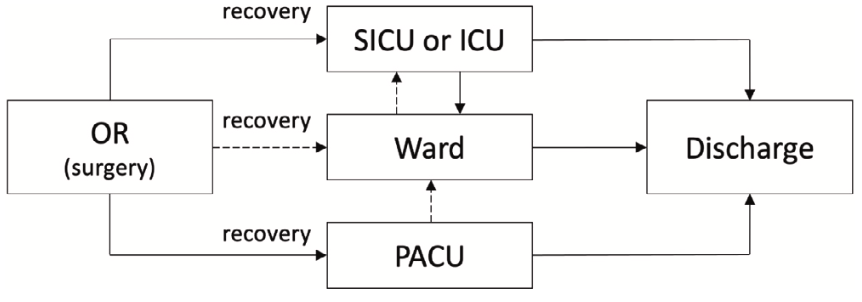
\includegraphics[width=.7\textwidth]{figures/SR0015US22/fig1.png}
        \caption{Potential patient flow in \cite{x335}.}
        \label{fig1:SR0015US22}
    \end{figure}
    
    \textbf{Page 3 (Introduction):}
    This paper does not consider emergency surgeries. The focus of the review lies in on the OR scheduling with downstream capacity, any papers that go beyond this critaria re out of scope of this research. The outline of the work finalyses the introduction section.

    \textbf{Page 3 (Impact of uncertainty):}
    The parameters of the uncertainties in OR scheduling will be introduced further in this section. \underline{fluctuating surgery duration}: ~surgeon workload, ~surgery work-content such as surgery type, surgery sequence, priority constraints, degree of timeoverlap between surgeries (refs). The duration is often an input parameter for scheduling algorithms. \underline{Length of Stay}: related to SICU (days), inpatient wards (days), and PACU (hours), and depends on ~surgery type, ~anaesthetics, ~patient. Surgery cancellation leads not only to financial loss, but also to worsenning the health state for patients.

    \textbf{Page 4 (Impact of uncertainty):}
    \dots PACU is known as a bottleneck of the surgeries flow in hospitals. 20-hour PACU blocking caused up to ~\$44,000 for a pediatric hospital in California (not including overtime costs, additional revenue losts from following cancellations). /underline{Impact and challenges of multimodality}: most of the papers doew not consider uncertainty of the scheduling problem, most of which is due to unability to access real hospital records. According to data of the Erasmus University Medical Center the durations of the surgeries are fluctuating and not uniformally. It is impossible to know whether or not the complecations occure during the surgery operation. Therefore, papers which are not considering uncertainty are suboptimal. \underline{Opportunities for modeling uncertainty}: by improving IT systems in hospitals, for example, by using RTLS systems. The EHRs are still under development and in process of addoptimng for many hospitals. There is a study on FJSS implementation inte hospital information and management system (HIMS).
    \begin{figure}[H]
        \centering
        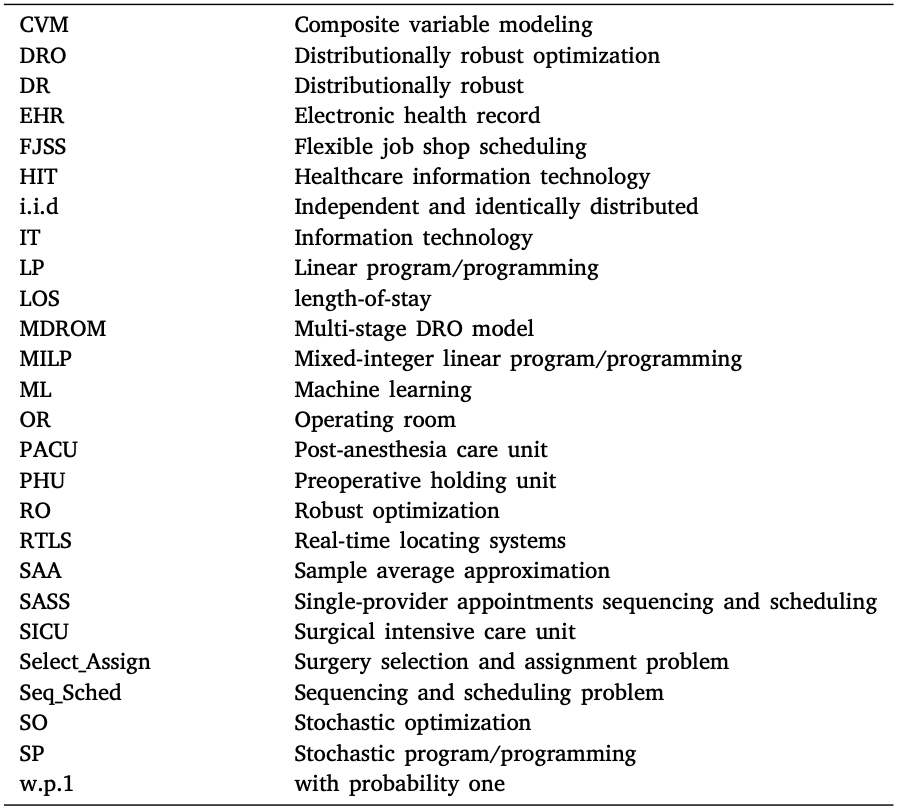
\includegraphics[width=.9\textwidth]{figures/SR0015US22/fig2.png}
        \caption{Acronyms in \cite{x335}.}
        \label{fig2:SR0015US22}
    \end{figure}
    \begin{figure}[H]
        \centering
        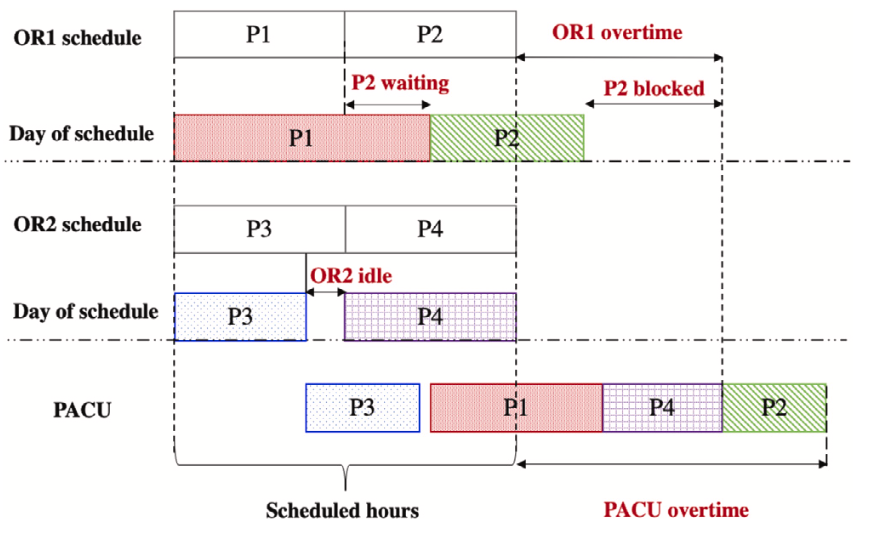
\includegraphics[width=.9\textwidth]{figures/SR0015US22/fig3.png}
        \caption{Two-OR and one-PACU patient flow from \cite{x335}.}
        \label{fig3:SR0015US22}
    \end{figure}

    \textbf{Page 5 (Stochastic optimisation):}
    There are three diractions to handle uncertainty in the scheduling problem: stochastic programming (SP), robust optimisation (RO), and distributionally robust optimisation (DRO). The short comaprison of the three diractions will be presented in this section. SP is efficient tool until the number of variables is low, when it is a lot of variations, the problem becomes exponantialy hardert to solve. To simplify the calculations, some authors resort to Monte Carlo simulation, which reduces number of solutions it tries to render. Then the authors proposed literature on techinal details of the sample average approximation (SAA). Next the robust optimisation is explaint in math terms. DRO is presented as in-between SP and RO methods...  
    \begin{figure}[H]
        \centering
        \frame{
            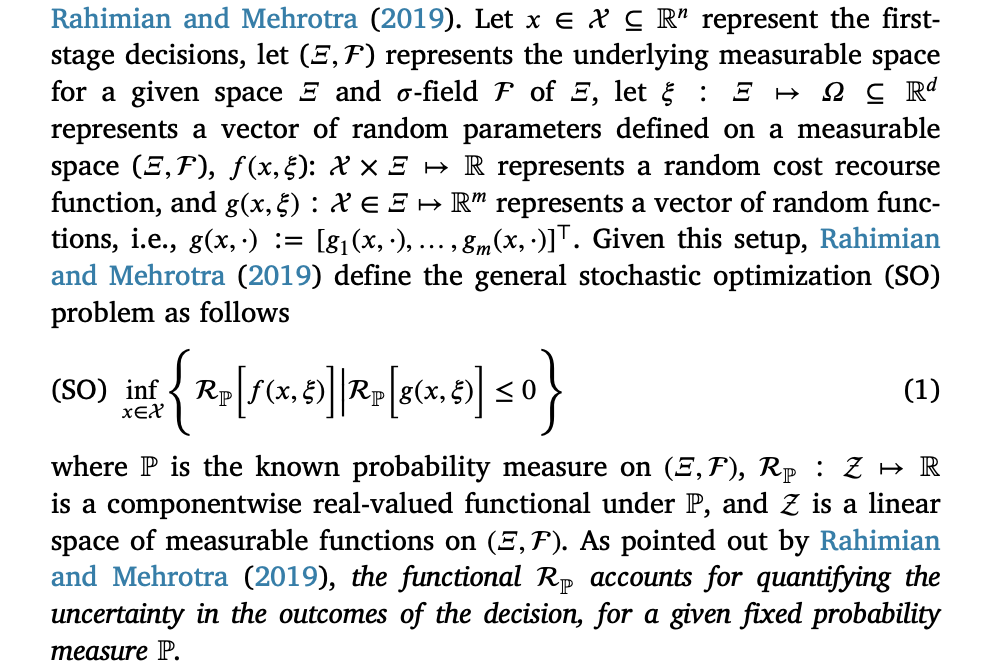
\includegraphics[width=.85\textwidth]{figures/SR0015US22/fig4.png}
        }
        \caption{Mach definition of the scheduling problem from \cite{x335}, SP part I.}
        \label{fig4:SR0015US22}
    \end{figure}
    \begin{figure}[H]
        \centering
        \frame{
            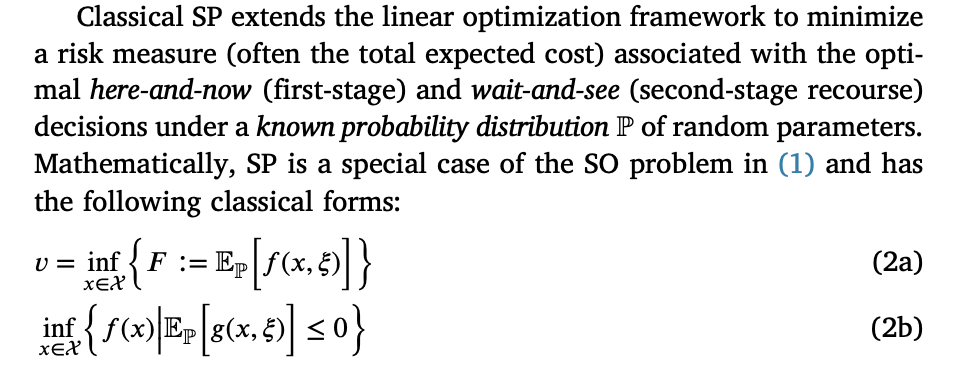
\includegraphics[width=.85\textwidth]{figures/SR0015US22/fig5.png}
        }
        \caption{Mach definition of the scheduling problem from \cite{x335}, SP part II.}
        \label{fig5:SR0015US22}
    \end{figure}
    \begin{figure}[H]
        \centering
        \frame{
            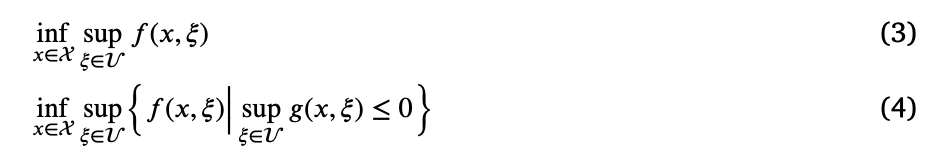
\includegraphics[width=1\textwidth]{figures/SR0015US22/fig6.png}
        }
        \caption{Mach definition of the scheduling problem from \cite{x335}, RO.}
        \label{fig6:SR0015US22}
    \end{figure}
    \begin{figure}[H]
        \centering
        \frame{
            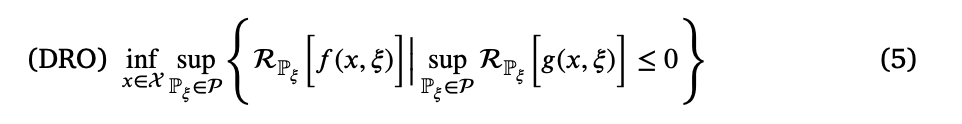
\includegraphics[width=1\textwidth]{figures/SR0015US22/fig7.png}
        }
        \caption{Mach definition of the scheduling problem from \cite{x335}, DRO.}
        \label{fig7:SR0015US22}
    \end{figure}

    \textbf{Page 6 (Stochastic optimisation):}
    ... more of DRO explanation in math term.

    \textbf{Page 6 (Modeling elective surgery scheduling problem):}
    The outline of the researched model of stochastic optimisational surgery scheduling with downstream capacity. Each specialty has its own block of time. Two stage planning: assign surgeries to the blockes, sequencing (allocating) start times of the surgeries. \underline{Typical performance metrics}: cost of performing/ postponing surgeries, percentage of scheduled surgeries, OR idle and overtime, recovery unit utilisation, premature SICU transfer, OR blocking time, surgery cancellation and delay, OR and recovery units congestion, and clinical staff workload, and even more metrics in references. These is no knowned approach which can solve the scheduling with all this metrics combined, so researchers desided to divide and conter the problem into smaller dyjastible parts. \underline{Select\_Assign}: From I waiting list to B surgery blocks + downstream capacity. Performing/ delaying a surgery has a cost. Math formulation of the problem. \underline{SP approaches for Select\_Assign}: SP formulation with two costs and math model...

    \textbf{Page 7 (Modeling elective surgery scheduling problem):}
    ... Starts with the list of studies. \underline{SP Solution Approaches and Challenges}. Stochastic SP is replaces by deterministic MILP in two steps: select N samples with independent surgery duration and LOS; sample average of thses samples. \underline{Large scale SAA-MILP formulations}. With bigger problem the sample size will also grow, therefore sometimes spliting problem into smaller chunks with other mathematical approaches may resolvethis issue. \underline{Symmertry}. Simmetricaly good solutions also have their caviate: there are more local optima which can trap the progress of optimisational algorithms.
    
    \textbf{Page 8 (Modeling elective surgery scheduling problem):}
    \underline{Distribution Anbinquity}. The assamption of the certain duration hurts SP ability to preform well even in idealised scenarios. \underline{RO approaches for Select\_Assign}. The high scheduling time for small problems too. Unable to capture the uncertainty distribution. \underline{DRO approaches for Select\_Assign}. Removes non-realistic assumptions about disctribution of uncertainty for LOS and surgery duration. Better then RO. Succesfull applications. The idel time cost is a critical parameter in operating room scheduling (~\%37.45, Rocherster Medical Centre California). The patient sutisfaction is another important metric.

    \textbf{Page 9 (Modeling elective surgery scheduling problem):}
    ... some more examples of implementing DRO. \underline{Opportunities}: data-driven DRO are both "tractable" and "implementable". Next author describe the implementability but through ambiquity with math model...
    \begin{figure}[H]
        \centering
        \frame{
            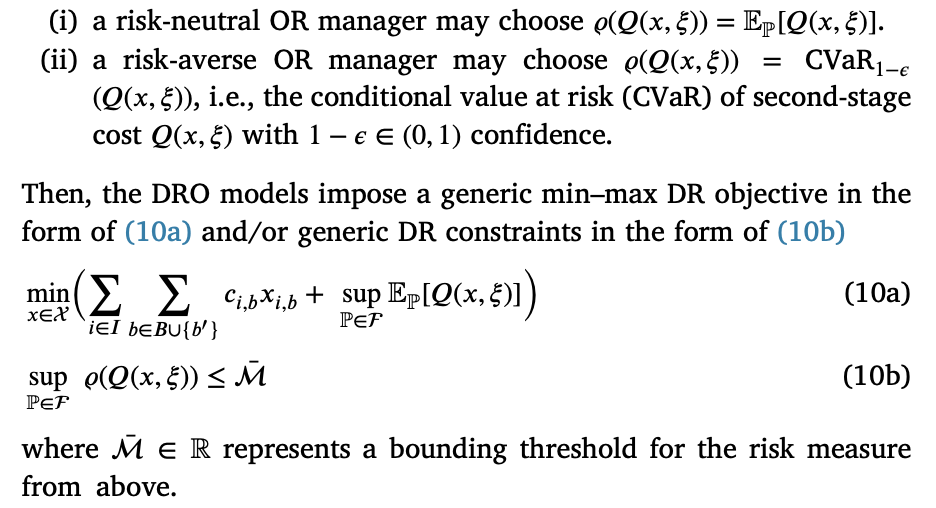
\includegraphics[width=.85\textwidth]{figures/SR0015US22/fig8.png}
        }
        \caption{DRO Select\_Assign Model from \cite{x335}.}
        \label{fig8:SR0015US22}
    \end{figure}

    \textbf{Page 10 (Modeling elective surgery scheduling problem):}
    ... some examples from literature. \underline{Solution methods}: there are easy to implement specific algorithm which require fine tuning and "hand work"; however the authors aim for more robust solution which will not require reassembling for each specific problem (Goh abd Sim, 2010). "For example, one can solve a more restricted version of the problem called affinely adjustable robust counterpart (AARC). Tractable DRO heuristics like AARC with distributional ambiguity has not been investigated for this class of problems." (reflection: decided to go with quotation, because do not exactly understand what is going on here). In addition, the authors propose combine computational efficiency of and solution quality. (reflection: do not quite understand how. What components will ensure one and the other? AARC - efficiency and DRO - quality of solution?). 
    
    \underline{Surgery Sequencing and Scheduling Problem (Seq\_sched)}: After the assigment of the surgery cases from waiting list was done, a hospital manager allocate the surgeries in sequence by the start time. \underline{SO approaches for Seq\_Sched with SICU/ ward capacity}: Sequencing = single-provider SASS (Stochastic Appointment Sequencing and Scheduling). SASS is widely research complex stochastic combinatorial optimisation problem. Resetnly a novel SP solution was developed to enhance SASS. Some more literature that the author suggest to readers. \underline{SO approaches for Seq\_Shed with PACU capacity}: PACU are often overvelmed in high-paith scenario when surgery time is less then the patients recovery time. PACU $~>$ OR scheduling $=>$ downstream capacity blocking. Another direct voice of the author "Note that blocking is not clinically feasible for surgeries that require recovery in SICU because it is not possible to hold a patient in the OR for several days after surgery until a SICU bed becomes available." (reflaction: is it just theoretical assumtion?).
    
    \textbf{Page 11 (Modeling elective surgery scheduling problem):}
    ... PACU admission policy can also be a constrain (i.e. what patient has a priority if two surgeries finishe at the same time?). \underline{Existing SO approaches}:PACU metricies: patient waiting time, OR blocking time, OR finish and idel times. PACU staff overtime, and surgery cancellation. There are only two publications which cover multiple objectives at once (Table A.1 Appendix). Next three examples of Seq\_sched PACU are discussed. \underline{Opportunity}: The authors offered to analyse upper boundary for the PACU blocking time, since it it impossible completelly illiminate downstream blocking. In addition, the patient admission PACU policy such as FCFS (FIFO) and Critica-Patient-First (CPF) are prooved sibotimal approaches which can be enhanced. Then the authors propose an methods to deel with probable obsticles: (a) Composite Variable Modeling is a known method to reduce the size, remove complex objectives, and empover the LP relaxation of combinatorial optimisational problems; (b) Variable transformation - change how the LOS is represented in programming model; (c) Two-Stage Approximation - estimate scheduling by claculating it and comparing it within two policies: FCFS (FIFO) and (CPF). The final suggestion goes as a reminder of comparing the worst, and normal scenarios to render an optimsal scheduling considering both possible outcomes.
    \begin{figure}[H]
        \centering
        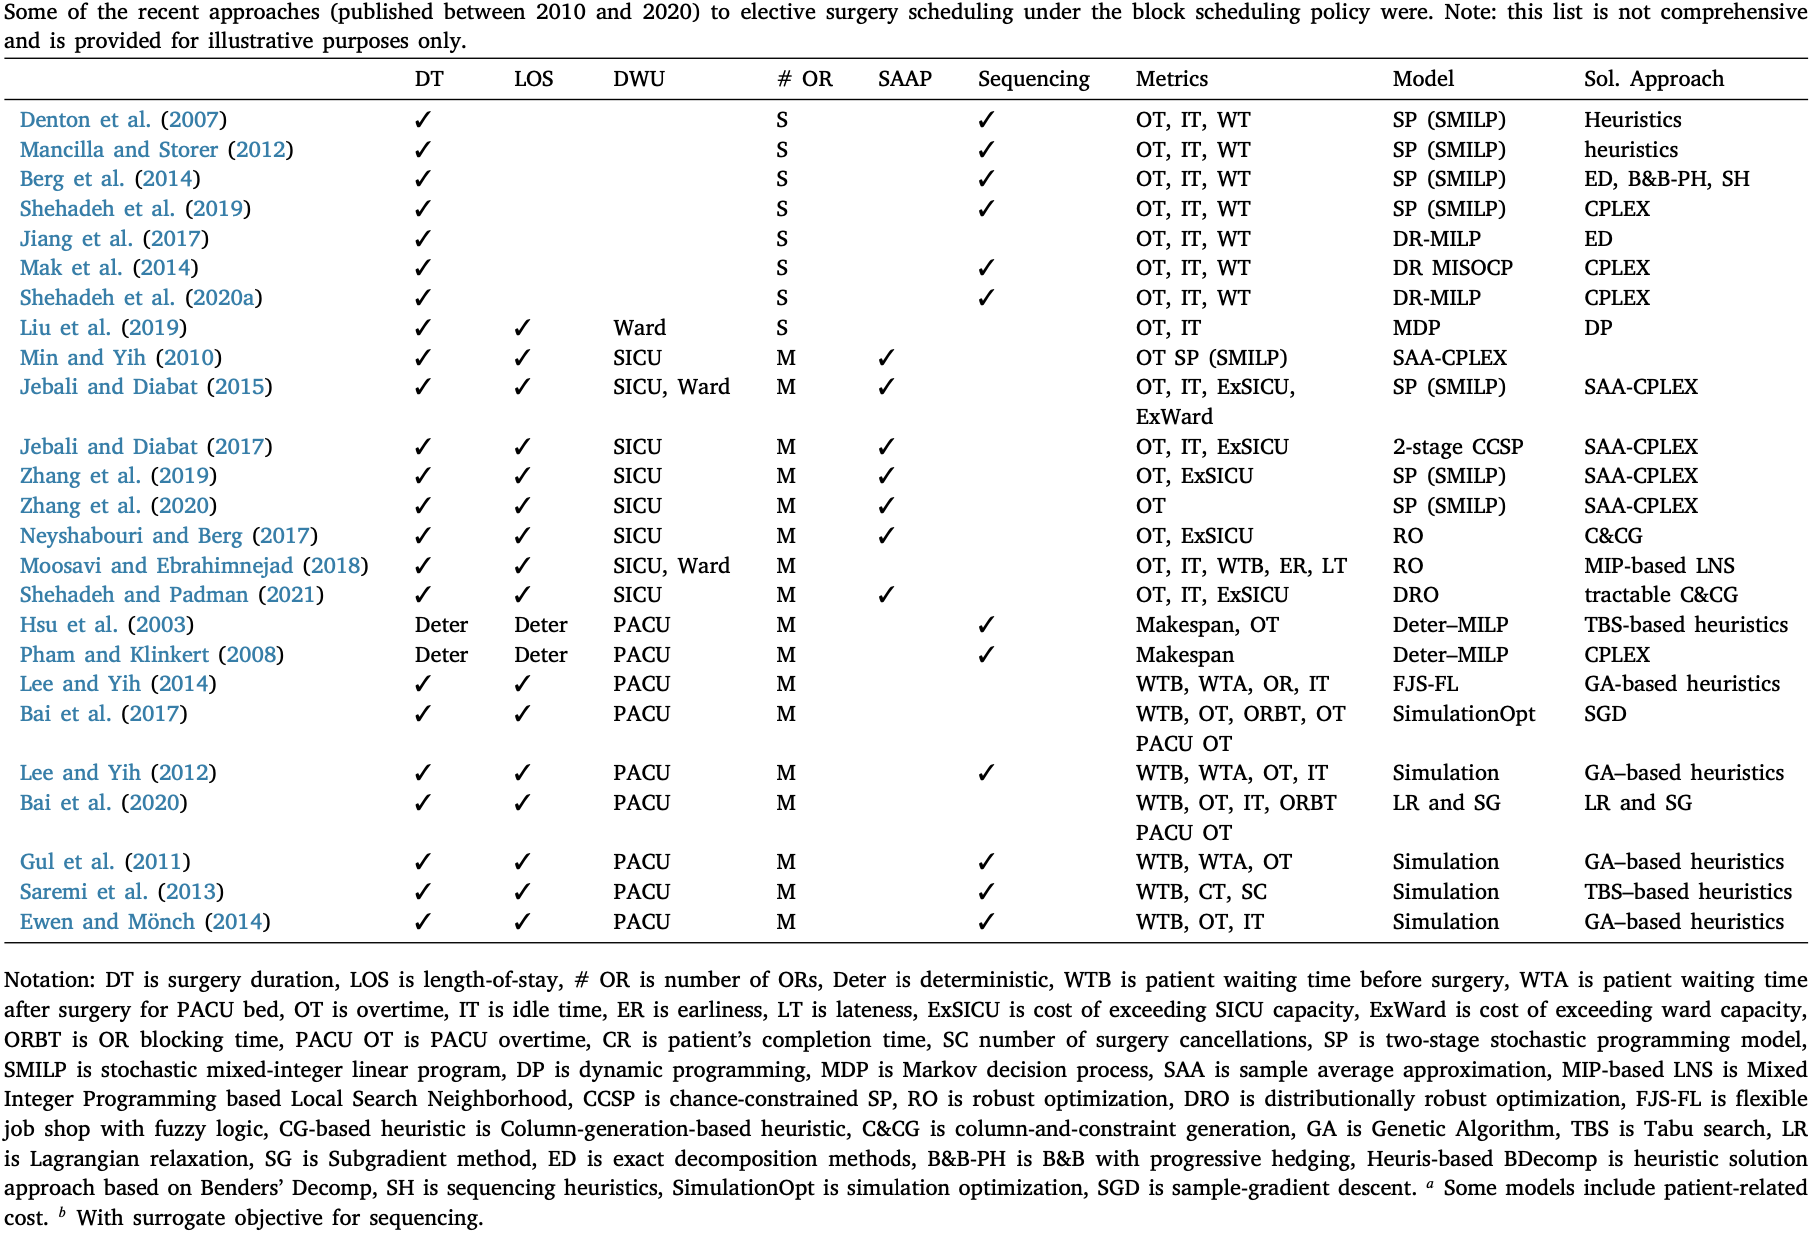
\includegraphics[width=1\textwidth]{figures/SR0015US22/fig9.png}
        \caption{Appendix from \cite{x335}.}
        \label{fig9:SR0015US22}
    \end{figure}

    \textbf{Page 12 (Future Research):}
    There are a lot of research in this field, but need more and better. \underline{Elective Surgery Databases}: There is a lot of medical records on surgery operation and PACU but it is no use unless it is preprocessed and stored in unified database system. The policy for structured data recording systems is required. The authors suggested to increase number of hospitals which use IT systems such as RTLS to track the capacity and resource availability (reflection: ask Anton for his londary project about RTLS). Enphasis of diversity of the origins of the timely records.
    
    \textbf{Page 13 (Future Research):}
    \underline{Exploiting the Power of ML}: Nowadays ML are efficient in solving tasks which envolve a big samples of data (the examples presented next). The downstide of the ML is their unpredictability and, relatively to defined methods, low accuracy. Sinse ML are hardly related to data to perform well, the best approach to generalise the ML model is to ensure that the process of building and adjusting ML in new envormenet can be replicated. Another good diraction is researching the adaptible ML (with self-tuning parameters). \underline{The Multi-Criteria and Cost Estimated Dilemma}: Current multi-objective optimisation solutions articulate with multi-objective functions to design a scheduling. In reality, the objective types are fluid and can change overtime, which makes it harder for desicion-makers to use the MOOs. Some objectives are hard to specifically define and others are closely interconnected, which is also hard to treck. Therefore, sugested future research shold focus on narrowing the gap between MOO and real-world implementation as well as with balancing between expances, resource usage, and capacity... 
    
    \textbf{Page 14 (Future Research):}
    ... \underline{Preoperative activities, unpunctuality, and no-show}. There is a flow of processes before an actual knife-to-skin surgery. The flow is different for inpatients and outpatients. PHU also can become a bottleneck. The patient latency and no-shows are sufficiently impact the flow of the surgeries further in the queue. \underline{Integrated approaches}: The authors underline an importane of easy-to-use integrated desicion support tool for operating hospitals. "Some of the existing formulations often rely on big-M coefficients that take large values and undermine computational efficiency. Big-M is often used to relax some of the constraints or en- force certain conditions, among other uses (e.g., ensure that the waiting time of a patient is zero when the patient is not scheduled). Camm et al. (1990) provide specific guidance for practitioners interested in the ubiquitous big-M and provide many practical examples to demonstrate that almost always, there is a maximum theoretical and practical size for the big-M coefficients that can be derived using the structural properties of the problem. Such a smart choice of big-M value could improve the model solvability compared to using unnecessarily large values for this parameter, diminishing model tractability" (reflection: I copy the chunk of the paper again, since do not understand it). This scheduling task requires gread deel of coordination between the objectives. The available studies layed a good foundation for further scheduling solution development. \underline{Capacity planning during the period of high demand}: Even advanced desicion support systems can not help if there is not enough well trained medical personnel, which was easy comfirmed by COVID19 crisis. There is yet to be more consideration what policy to follow in times of critical demand. Just increasing the number of ICU beds will not always an effective solution. There is already some studies in this diration.

    \textbf{Page 15 (Future Research):}
    \underline{Decision support tools}: A developed desicion support system should be effective and user-friendly. The proposedworkbanch E-HOSPITAL supports three level of desicion making and has several problems which can be solved. This tool is digital and is available for stakeholders and in pedagogical staff (healthcare analytics, service management, and information systems).

    \textbf{Page 15 (Conclusions):}
    The curent review demonstrats a research on optimal stochastic elective surery scheduling with downstream capacities. The authors focus on three main approaches in the field: SP, RO, and DRO for the last decade (2010-2020). The uncertain surgery duration and postoperative LOS are critical criteria for consideration in effective scheduling advisory systems. Crusial points: (a) Lack of data-driven approaches; (b) There is no model which solves selection and assignment problems at the same time; (c) Lack of research which acknowledge the stohastic nature of the surgery duration and LOS, and consider the multimodal distribution of the durations; (d) There is great number of interconnected contraints, therefore no solution which can deel with all of them at once.(e) Scheduling considering SICU is easier and more researched than scheduling with PACU. (f) The authros proposed a few approaches which can overcome existing obsticles. Authors' suggestions: (1) Develop unified healthcare record system; (2) design data-driven ML- and optimisation-based approaches; (3) develop user-friendly and implementable tool for effective decision making; (4) consider methods for high-demand scenarios.